\documentclass[10pt,a4paper]{article}

\usepackage[T1]{fontenc}
\usepackage[utf8]{inputenc}
\usepackage[provide=*,main=portuguese]{babel}
\usepackage{lmodern}
\usepackage{geometry}
\usepackage{amsmath,amssymb}
\usepackage{booktabs}
\usepackage{tabularx}
\usepackage{array}
\usepackage{enumitem}
\usepackage{graphicx}
\usepackage{float}
\usepackage{xcolor}
\usepackage{listings}
\usepackage[hidelinks]{hyperref}
\usepackage{microtype}
\usepackage[round,authoryear]{natbib}
\setcitestyle{open={[},close={]},aysep={ },yysep={,},citesep={, }}
\usepackage{tikz}
\usetikzlibrary{positioning}
\usepackage{pgfplots}
\pgfplotsset{compat=1.18}

\geometry{top=2.2cm,bottom=2.2cm,left=2.3cm,right=2.3cm}
\setlength{\parindent}{1.0cm}
\setlength{\parskip}{0.2em}
\renewcommand{\arraystretch}{1.1}
\newcommand{\articletitle}{Análise de Desempenho de Servidores RTMP e Transcodificadores no Streaming de Vídeo}

\lstset{basicstyle=\ttfamily\small,breaklines=true,frame=single}

\begin{document}

\begin{center}
  \vspace*{-0.8cm}
  \parbox{0.92\textwidth}{
    \centering
    {\Large\bfseries \articletitle\par}
    \vspace{0.45cm}
    {\normalsize Valter Abreu Silva Júnior\textsuperscript{1}, Prof. Dr. Mário Antônio Meirelles Teixeira\textsuperscript{2}\par}
    \vspace{0.08cm}
    {\small Departamento de Informática -- Universidade Federal do Maranhão (UFMA)\par}
    {\small Av. dos Portugueses, 1966 -- Cidade Universitária Dom Delgado\par}
    {\small 65080-805 -- São Luís -- MA -- Brasil\par}
    {\small valter.abreu@discente.ufma.br, mario.teixeira@ufma.br\par}
  }
  \vspace{0.35cm}
\end{center}

\noindent\textbf{Abstract.} This paper presents an experimental study on the performance of RTMP servers and video transcoders in a live streaming platform. The implemented platform combines Nginx-RTMP or SRS for ingestion, FFmpeg or GStreamer for transcoding, and HLS for browser delivery. A $2\times2\times3$ factorial design was executed with four technology combinations, loads of 1, 10, and 50 synthetic viewers, and three repetitions per treatment. The analysis considers master-playlist startup time, CPU and memory consumption, effective bitrate, HTTP request error rate, and container restarts. The results indicate that SRS made the HLS master playlist available earlier in the evaluated environment, while GStreamer used less memory and, in some combinations, exerted greater CPU pressure. The measured end-to-end latency is treated as an invalidated proxy rather than conclusive evidence, because the benchmark does not yet synchronize publication, segment generation, delivery, and playback timestamps.

\noindent\textbf{Keywords:} video streaming; RTMP; transcoding; FFmpeg; GStreamer; performance; HLS.

\noindent\textbf{Resumo.} Este artigo apresenta um estudo experimental sobre o desempenho de servidores RTMP e transcodificadores em uma plataforma de streaming de vídeo ao vivo. A plataforma implementada combina Nginx-RTMP ou SRS para ingestão, FFmpeg ou GStreamer para transcodificação e HLS para entrega ao navegador. Foi executado um delineamento fatorial $2\times2\times3$, com quatro combinações tecnológicas, cargas de 1, 10 e 50 espectadores sintéticos e três repetições por tratamento. A análise considera o tempo de disponibilização da playlist mestre, o consumo de CPU e memória, o bitrate efetivo, a taxa de erros de requisições HTTP e os reinícios do container. Os resultados indicam que o SRS disponibilizou a playlist mestre mais cedo no ambiente avaliado, enquanto o GStreamer consumiu menos memória e, em algumas combinações, exerceu maior pressão sobre a CPU. A latência ponta a ponta medida é tratada como um proxy não validado, pois o benchmark ainda não sincroniza os timestamps de publicação, geração do segmento, entrega e reprodução.

\noindent\textbf{Palavras-chave:} streaming de vídeo; RTMP; transcodificação; FFmpeg; GStreamer; desempenho; HLS.

\section{Introdução}

O streaming ao vivo exige que uma cadeia de processamento receba o vídeo, transforme-o em representações adequadas e o entregue aos espectadores com continuidade e atraso reduzido. Nessa cadeia, o servidor de ingestão e o transcodificador podem consumir recursos de forma diferente e introduzir atrasos distintos. A escolha entre alternativas aparentemente equivalentes, portanto, deve ser apoiada por medições reproduzíveis, e não apenas por disponibilidade de documentação ou popularidade.

O projeto deste trabalho implementa uma plataforma de streaming composta por frontend, backend de controle, servidor RTMP, transcodificador e entrega HLS. O desenho permite alternar o servidor entre Nginx-RTMP e SRS e o transcodificador entre FFmpeg e GStreamer, mantendo a aplicação e o conteúdo de teste sob controle. Essa característica torna possível investigar o efeito da combinação dos componentes sobre uma mesma carga de trabalho.

O problema de pesquisa é: \textit{como as combinações de servidores RTMP e transcodificadores influenciam o desempenho, o consumo de recursos e a estabilidade de uma plataforma de streaming de vídeo ao vivo em um ambiente conteinerizado?}

\subsection{Objetivo geral}

Avaliar o desempenho de servidores RTMP e transcodificadores no streaming de vídeo, comparando Nginx-RTMP e SRS combinados com FFmpeg e GStreamer em cargas controladas.

\subsection{Objetivos específicos}
\begin{itemize}[leftmargin=1.2cm]
  \item Descrever a arquitetura implementada e o fluxo RTMP--transcodificação--HLS.
  \item Definir uma matriz experimental que permita comparar servidor, transcodificador e número de espectadores.
  \item Medir tempo de disponibilização, CPU, memória, bitrate, erros de entrega e reinícios.
  \item Analisar a estabilidade dos cenários por médias e desvios padrão de três repetições.
  \item Identificar limitações da instrumentação e propor melhorias para uma avaliação posterior.
\end{itemize}

\subsection{Contribuições}
\begin{itemize}[leftmargin=1.2cm]
  \item Uma plataforma de streaming configurável e executável por Docker Compose.
  \item Um benchmark automatizado com dados brutos, logs e agregação estatística.
  \item Uma comparação experimental entre quatro combinações de software sob três cargas.
  \item Uma análise explícita das limitações de validade dos resultados disponíveis.
\end{itemize}

\subsection{Organização do trabalho}

O texto está organizado em seis seções principais. A Seção 2 apresenta os trabalhos relacionados; a Seção 3 descreve a metodologia; a Seção 4 apresenta e discute os resultados; a Seção 5 conclui o estudo e indica trabalhos futuros; e a Seção 6 reúne as referências utilizadas.

\section{Trabalhos Relacionados}

Estudos de desempenho em sistemas de streaming normalmente observam atraso, continuidade da reprodução, qualidade percebida, vazão e consumo de recursos. A literatura de streaming adaptativo destaca que o comportamento percebido pelo usuário resulta da interação entre qualidade de vídeo, variações de bitrate, tempo de início e interrupções \cite{seufert,barman}. Neste trabalho, o foco é anterior à decisão adaptativa do cliente: avaliar como a ingestão RTMP e a geração das representações HLS afetam o comportamento do serviço.

Seufert et al. apresentam uma revisão de qualidade de experiência em HTTP Adaptive Streaming, discutindo fatores técnicos e perceptuais associados à adaptação de vídeo. Barman e Martini ampliam essa discussão ao revisar modelos de QoE e desafios de avaliação. Esses trabalhos orientam a seleção de métricas relacionadas à experiência, mas não comparam diretamente as quatro combinações implementadas neste projeto.

Em relação a protocolos, a especificação do RTMP descreve um protocolo de aplicação baseado em transporte confiável, adequado à multiplexação de áudio, vídeo e dados \cite{rtmp}. O HLS, por sua vez, organiza a apresentação em playlists e segmentos acessíveis por HTTP \cite{hls}. A solução avaliada usa RTMP na publicação e HLS na distribuição, refletindo uma arquitetura comum de ingestão e entrega desacopladas.

As documentações oficiais do FFmpeg e do GStreamer descrevem mecanismos diferentes de composição de pipelines \cite{ffmpeg,gstreamer}. FFmpeg oferece uma ferramenta integrada para demux, filtros, codificação e mux; GStreamer organiza o processamento como uma cadeia de elementos conectados. A comparação deste trabalho não pretende declarar um transcodificador universalmente superior, pois os resultados dependem das versões, parâmetros, número de variantes e hardware utilizados.

A principal lacuna abordada é a comparação controlada entre servidor RTMP e transcodificador na mesma plataforma, com a mesma entrada, parâmetros de saída e cargas de espectadores. O uso de containers favorece a repetição do ambiente \cite{docker}, enquanto Nginx-RTMP e SRS fornecem as alternativas de servidor avaliadas \cite{nginxrtmp,srs}. O benchmark automatizado e os artefatos versionados aproximam o estudo de uma avaliação reprodutível, mas seus resultados permanecem limitados ao ambiente documentado.

\subsection{Síntese da lacuna}

Os trabalhos consultados oferecem fundamentos para protocolos, QoE e ferramentas multimídia. Contudo, não respondem diretamente qual combinação Nginx-RTMP/SRS e FFmpeg/GStreamer apresenta melhor comportamento sob as cargas definidas. A contribuição experimental deste TCC é preencher esse recorte com uma matriz comparável e explicitar as métricas que ainda não foram instrumentadas adequadamente.

\section{Metodologia}

Foi adotada uma abordagem quantitativa, experimental e comparativa. O fator servidor possui dois níveis (Nginx-RTMP e SRS), o fator transcodificador possui dois níveis (FFmpeg e GStreamer) e a carga possui três níveis (1, 10 e 50 espectadores sintéticos). O delineamento fatorial $2\times2\times3$ resulta em 12 tratamentos, cada um repetido três vezes, totalizando 36 execuções. A unidade experimental é uma sessão completa de publicação, transcodificação e leitura HLS executada em um ambiente reconstruído pelo Docker Compose.

\begin{table}[H]
\centering
\caption{Fatores e níveis do experimento}
\begin{tabularx}{\textwidth}{@{}lXX@{}}
\toprule
Fator & Níveis & Papel no experimento \\
\midrule
Servidor RTMP & Nginx-RTMP; SRS & Recebe a publicação RTMP e dispara o processamento \\
Transcodificador & FFmpeg; GStreamer & Gera as variantes HLS \\
Carga & 1; 10; 50 viewers & Simula demanda crescente de leitura \\
Repetição & 3 por tratamento & Permite estimar média e desvio padrão \\
\bottomrule
\end{tabularx}
\end{table}

\subsection{Arquitetura e fluxo experimental}

No benchmark, uma fonte sintética é gerada pelo container \texttt{jrottenberg/ffmpeg:6.0-alpine} com o padrão \texttt{testsrc} em 1280$\times$720 a 30 quadros por segundo, acompanhada por um sinal de áudio senoidal. O publicador envia essa fonte por RTMP ao servidor selecionado. Nginx-RTMP ou SRS aciona o script do transcodificador, que lê o fluxo RTMP, codifica quatro variantes e grava playlists e segmentos HLS. Os viewers sintéticos são containers \texttt{curlimages/curl:8.7.1}; cada um requisita a playlist mestre, uma playlist de variante e o segmento mais recente em ciclos de um segundo. O backend Spring Boot, PostgreSQL, RabbitMQ e frontend fazem parte da aplicação, mas o alvo principal da medição de CPU e memória é o container RTMP/transcodificador.

\begin{figure}[H]
\centering
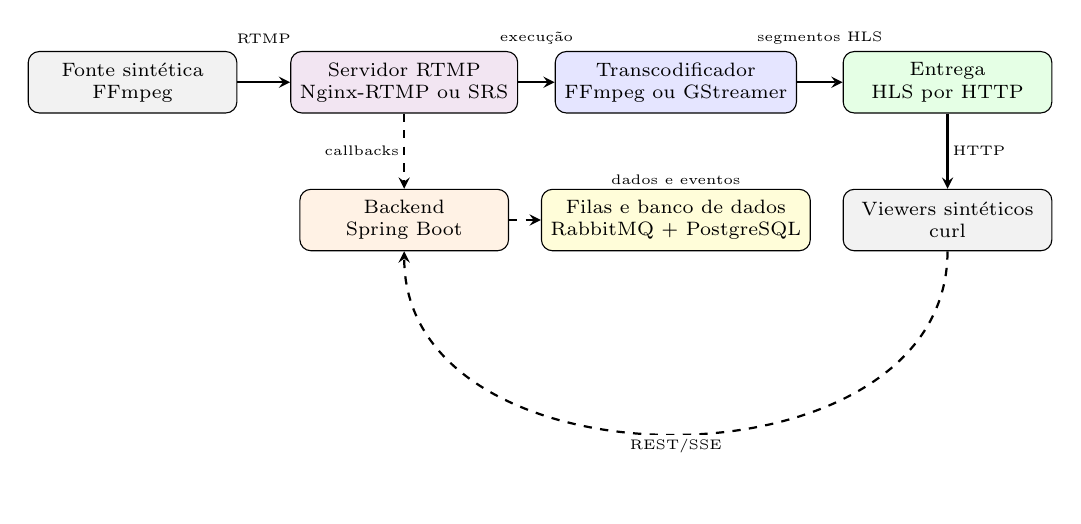
\begin{tikzpicture}[
  box/.style={draw, rounded corners, align=center, minimum width=2.65cm, minimum height=0.78cm, font=\scriptsize},
  arrow/.style={->, thick, >=stealth},
  label/.style={font=\tiny, fill=white, inner sep=1.5pt}
]
\node[box, fill=gray!10] (obs) at (0,0) {Fonte sintética\\FFmpeg};
\node[box, fill=violet!10] (rtmp) at (3.45,0) {Servidor RTMP\\Nginx-RTMP ou SRS};
\node[box, fill=blue!10] (trans) at (6.90,0) {Transcodificador\\FFmpeg ou GStreamer};
\node[box, fill=green!10] (hls) at (10.35,0) {Entrega\\HLS por HTTP};
\node[box, fill=orange!10] (backend) at (3.45,-1.75) {Backend\\Spring Boot};
\node[box, fill=yellow!15] (services) at (6.90,-1.75) {Filas e banco de dados\\RabbitMQ + PostgreSQL};
\node[box, fill=gray!10] (viewer) at (10.35,-1.75) {Viewers sintéticos\\curl};
\draw[arrow] (obs.east) -- node[above=0.42cm,label]{RTMP} (rtmp.west);
\draw[arrow] (rtmp.east) -- node[above=0.42cm,label]{execução} (trans.west);
\draw[arrow] (trans.east) -- node[above=0.42cm,label]{segmentos HLS} (hls.west);
\draw[arrow] (hls.south) -- node[right,label]{HTTP} (viewer.north);
\draw[arrow,dashed] (rtmp.south) -- node[left,label]{callbacks} (backend.north);
\draw[arrow,dashed] (backend.east) -- (services.west);
\node[anchor=south, label] at (services.north) {dados e eventos};
\draw[arrow,dashed] (viewer.south) to[out=270,in=270,looseness=1.15] node[below,label]{REST/SSE} (backend.south);
\end{tikzpicture}
\caption{Arquitetura experimental da plataforma.}
\end{figure}

\subsection{Interface da plataforma}

Além da infraestrutura de processamento, a plataforma possui uma interface web para criação de transmissões, consulta das lives disponíveis e acesso ao painel do publicador. A interface não é utilizada como instrumento primário de medição, mas demonstra o fluxo de uso que conecta a implementação experimental ao cenário de aplicação. O publicador cria uma transmissão, recebe os dados necessários para configurar o software de captura e acompanha o estado da sessão; o espectador acessa a transmissão pela página de reprodução.

\begin{figure}[H]
\centering
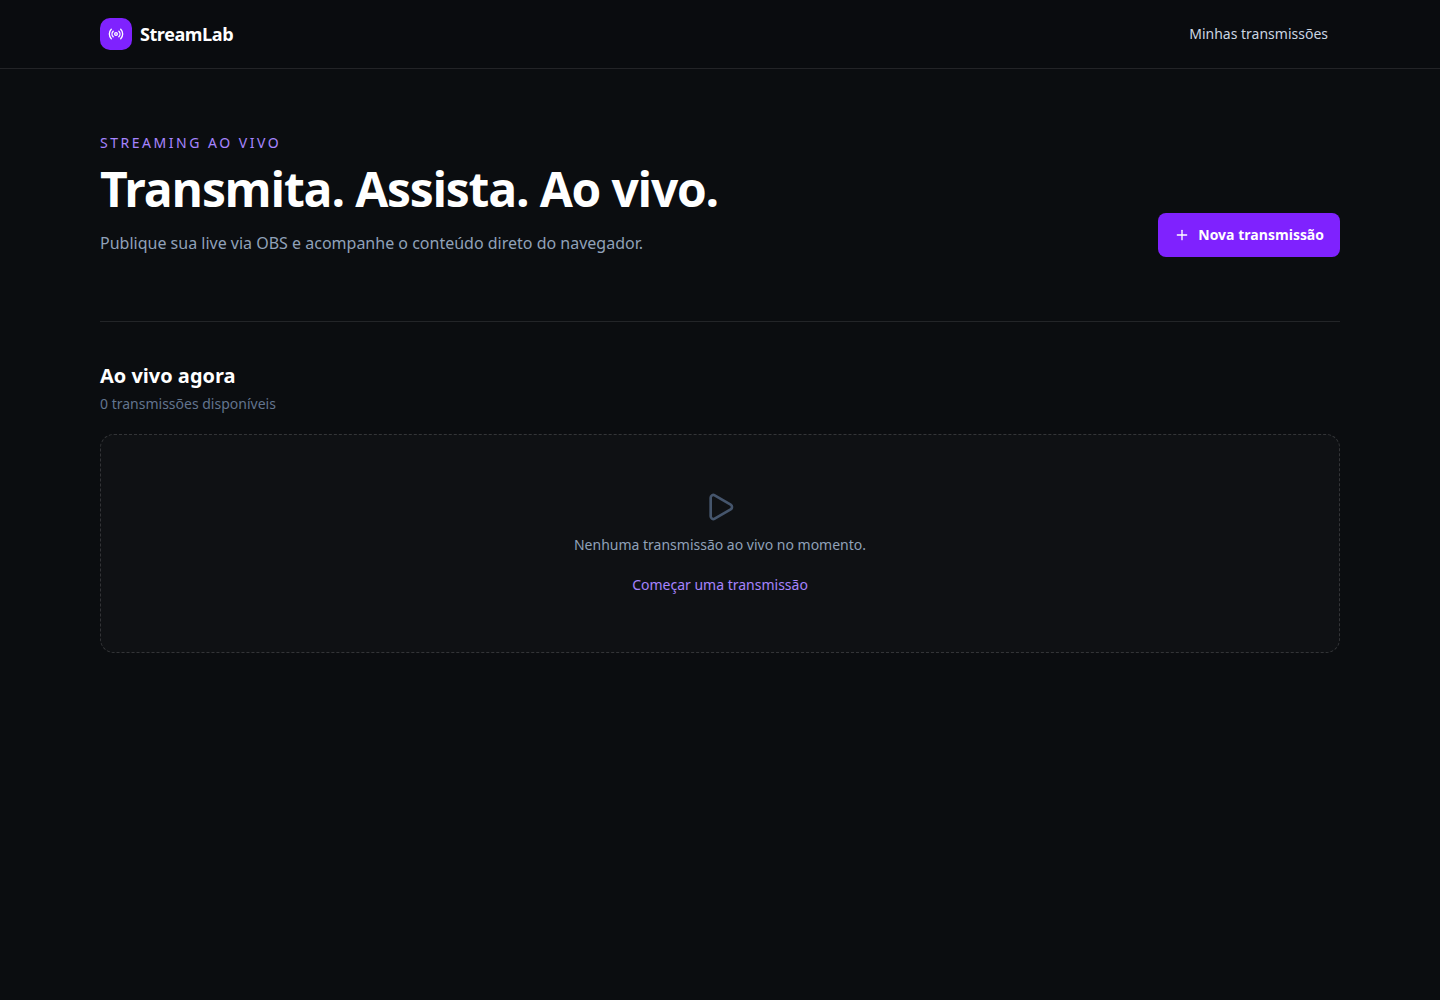
\includegraphics[width=0.94\textwidth]{../screenshots/home.png}
\caption{Tela inicial da plataforma de streaming.}
\label{fig:interface-home}
\end{figure}

A Figura~\ref{fig:interface-home} apresenta a tela inicial em seu estado sem transmissões ativas. A interface documenta a aplicação construída, mas não é usada como instrumento primário do benchmark. Dessa forma, os resultados quantitativos são produzidos pelos scripts automatizados, enquanto a figura evidencia a integração entre a infraestrutura avaliada e o cenário de uso da plataforma.

\subsection{Configuração do conteúdo e dos pipelines}

O FFmpeg gera quatro variantes (1080p, 720p, 480p e 360p) por meio de divisão do vídeo, redimensionamento, codificação H.264 e mux HLS \citep{ffmpeg}. Os alvos de vídeo são, respectivamente, 5000, 2800, 1400 e 800 kbps, com áudio de 128, 128, 96 e 96 kbps. O GStreamer executa quatro pipelines paralelos com \texttt{rtmpsrc}, decodificação, redimensionamento, \texttt{x264enc}, codificação AAC e \texttt{hlssink2} \citep{gstreamer,gstreamerhls}; seus alvos de vídeo são 5000, 2500, 1400 e 600 kbps, com os mesmos alvos de áudio. Portanto, os alvos agregados não são idênticos: aproximadamente 10,0 Mbps de vídeo no FFmpeg e 9,5 Mbps no GStreamer. Essa diferença é registrada como uma ameaça à comparabilidade e impede interpretar o bitrate como uma medida isolada de eficiência ou qualidade.

Em ambos os pipelines, a duração nominal dos segmentos HLS é de 6 segundos e a playlist mantém 10 segmentos. A codificação é realizada em CPU, sem aceleração por GPU. As quatro representações seguem o modelo de múltiplas qualidades do HLS, mas a ausência de uma normalização completa dos parâmetros significa que a comparação é entre as configurações implementadas no projeto.

\subsection{Métricas}

\begin{table}[H]
\centering
\caption{Métricas coletadas e interpretação}
\begin{tabularx}{\textwidth}{@{}lXX@{}}
\toprule
Métrica & Unidade & Definição operacional \\
\midrule
Startup da playlist mestre & s & Tempo até a playlist mestre responder HTTP 200 \\
CPU média/máxima & \% & Uso agregado do container RTMP durante a janela medida \\
Memória média/máxima & MB & Memória observada no container \\
Bitrate efetivo & kbps & Estimativa a partir dos segmentos HLS \\
Taxa de erros HTTP & \% & Requisições de playlist ou segmento com erro divididas pelo total \\
Reinícios & contagem & Diferença do contador de reinícios do container \\
Primeiro segmento / proxy E2E & s & Campo coletado, mas não validado por timestamps sincronizados \\
\bottomrule
\end{tabularx}
\end{table}

\subsection{Procedimento e análise}

Cada cenário derruba a execução anterior e sobe uma instância limpa do ambiente conteinerizado, cuja finalidade é isolar e reproduzir os serviços da aplicação \citep{docker}. Em seguida, cria-se uma transmissão, inicia-se a fonte sintética, mede-se o tempo até a playlist mestre responder, inicia-se a quantidade definida de viewers e coleta-se o estado do container com \texttt{docker stats} em intervalos de dois segundos. A sessão nominal dura 300 segundos. Os dados brutos são consolidados por uma rotina de agregação estatística, que calcula médias e desvios padrão agrupados por servidor, transcodificador e carga.

Os critérios operacionais adotados no benchmark são disponibilidade da playlist mestre em até 24 s, CPU média de até 240\% para 1 e 10 viewers e 280\% para 50 viewers, taxa de erros de até 1\% para 1 e 10 viewers e 3\% para 50 viewers, além de zero reinícios. Esses limites são critérios de aceitação do experimento local, não requisitos universais de streaming. O percentual de CPU é agregado pelo Docker e pode ultrapassar 100\% quando o processo utiliza múltiplas threads do host.

\subsection{Delineamento fatorial}

O experimento pode ser representado como um delineamento fatorial $2\times2\times3$. Os dois primeiros fatores são tecnológicos e o terceiro representa a carga. Essa organização permite observar tanto o efeito isolado de cada fator quanto a interação entre servidor e transcodificador. Por exemplo, um transcodificador pode apresentar determinado consumo quando associado ao Nginx e comportamento diferente quando associado ao SRS, ainda que a carga permaneça constante.

Para cada tratamento, as três repetições são executadas com a mesma configuração de entrada e duração nominal. A média representa o comportamento central, enquanto o desvio padrão indica a variação entre repetições. Como o número de repetições é pequeno, os desvios são usados de forma descritiva; não se pretende realizar inferência estatística forte ou atribuir significância causal às diferenças observadas.

\subsection{Controle de variáveis}

Foram mantidos constantes o host, o sistema operacional, o mecanismo de virtualização, a resolução da fonte sintética, a duração dos segmentos e os parâmetros de retenção da playlist. A variável independente principal é a combinação servidor--transcodificador; o número de espectadores funciona como fator de pressão. Como variáveis dependentes, foram observados o startup HLS, o uso de CPU e memória, o bitrate efetivo, a taxa de erros e os reinícios.

Essa separação é importante porque o bitrate produzido não deve ser interpretado isoladamente como indicador de eficiência. Ele também depende do número de variantes, das resoluções, dos bitrates-alvo e dos parâmetros do encoder. Assim, a comparação de consumo precisa ser lida junto com a configuração de saída e com a estabilidade da entrega.

\subsection{Ambiente experimental}

\begin{table}[H]
\centering
\caption{Características do ambiente experimental}
\begin{tabularx}{\textwidth}{@{}lX@{}}
\toprule
Componente & Configuração \\
\midrule
Sistema operacional & Ubuntu 24.04.3 LTS, arquitetura x86\_64 \\
Processador & Intel Core i5-13420H, 13ª geração, 12 threads \\
Memória & 24 GB de RAM \\
Armazenamento & SSD NVMe, aproximadamente 231 GB \\
Rede & Loopback e bridge do ambiente conteinerizado \\
Orquestração & Docker Engine e Docker Compose \\
Codificação & CPU, sem aceleração por GPU \\
\bottomrule
\end{tabularx}
\end{table}

O registro do ambiente é necessário porque os valores de CPU e memória não são propriedades isoladas dos servidores ou transcodificadores. O percentual de CPU observado no container pode ultrapassar 100\% quando mais de uma thread é utilizada, enquanto a memória deve ser interpretada em relação à capacidade total do host e aos demais serviços ativos. Essa preocupação é consistente com estudos de avaliação de containers, que tratam a infraestrutura e o tipo de carga como fatores inseparáveis da medição de desempenho \citep{shirinbab}.

\subsection{Reprodutibilidade}

Uma execução pode ser reproduzida seguindo a sequência de selecionar o perfil do servidor, selecionar o transcodificador, reconstruir os containers, criar a transmissão, iniciar a fonte sintética, aplicar a carga de viewers, coletar as séries temporais e repetir o tratamento. O benchmark mantém CSV bruto, logs por cenário, amostras de métricas e um CSV agregado. A execução analisada foi identificada pelo run id \texttt{bench-full-20260517-164317}; o estado do host e os parâmetros do pipeline devem ser mantidos junto desses artefatos para permitir auditoria.

\subsection{Validade e limitações}

Os resultados são internos ao host Ubuntu 24.04.3, Intel Core i5-13420H, 24 GB de RAM, SSD NVMe e Docker Engine. Não há rede externa, GPU, variação de codec, variação de resolução de entrada ou comparação com outros hosts. A latência ponta a ponta não foi instrumentada de forma válida: o script reutiliza a medição de primeiro segmento como proxy e os registros apresentam zeros na maior parte dos tratamentos. A playlist mestre responder não significa necessariamente que um segmento válido já esteja disponível nem que o player tenha iniciado a reprodução. Por isso, essa métrica não é usada como evidência conclusiva; trabalhos futuros deverão sincronizar timestamps entre publicação, criação do segmento, disponibilização HTTP e leitura pelo viewer.

\section{Resultados e Discussão}

Esta seção apresenta os resultados agregados das três repetições realizadas para cada tratamento experimental. Os valores reportados são médias; os desvios padrão foram calculados a partir das respectivas repetições. Os registros brutos foram preservados para auditoria e reprodutibilidade do experimento.

\begin{table}[H]
\centering
\scriptsize
\caption{Médias agregadas dos tratamentos}
\begin{tabular}{@{}llrrrrrr@{}}
\toprule
Servidor & Transcod. & Viewers & Startup (s) & CPU (\%) & RAM (MB) & Bitrate (kbps) & Erros (\%) \\
\midrule
Nginx & FFmpeg & 1 & 21,67 & 177,88 & 1658,06 & 3524,66 & 0,00 \\
Nginx & FFmpeg & 10 & 22,00 & 159,35 & 1679,64 & 3526,08 & 0,00 \\
Nginx & FFmpeg & 50 & 22,33 & 196,86 & 1640,75 & 3522,54 & 0,00 \\
Nginx & GStreamer & 1 & 22,00 & 233,44 & 657,02 & 5344,59 & 0,00 \\
Nginx & GStreamer & 10 & 22,00 & 243,48 & 623,47 & 5342,92 & 0,00 \\
Nginx & GStreamer & 50 & 22,00 & 292,13 & 629,52 & 5344,05 & 0,00 \\
SRS & FFmpeg & 1 & 8,00 & 195,32 & 1665,30 & 3155,57 & 0,00 \\
SRS & FFmpeg & 10 & 8,00 & 197,34 & 1678,86 & 3156,01 & 0,00 \\
SRS & FFmpeg & 50 & 8,00 & 215,74 & 1623,08 & 3157,79 & 0,00 \\
SRS & GStreamer & 1 & 1,00 & 207,80 & 642,26 & 5340,31 & 0,00 \\
SRS & GStreamer & 10 & 1,00 & 215,82 & 625,27 & 5338,16 & 0,00 \\
SRS & GStreamer & 50 & 1,00 & 192,35 & 500,90 & 5337,81 & 3,15 \\
\bottomrule
\end{tabular}
\end{table}

\subsection{Síntese dos achados}

Nos dados atuais, o SRS apresenta startup de playlist menor que o Nginx nos dois transcodificadores: 8 s contra aproximadamente 22 s com FFmpeg e 1 s contra 22 s com GStreamer. Essa vantagem deve ser descrita como vantagem de disponibilização da playlist, não como redução comprovada da latência percebida, pois a instrumentação de latência ponta a ponta é incompleta.

O FFmpeg consome aproximadamente 1,62--1,68 GB de memória média, enquanto o GStreamer fica aproximadamente entre 0,50 e 0,66 GB. Em contrapartida, o GStreamer apresenta maior CPU média, especialmente com Nginx: 243,48\% em 10 viewers e 292,13\% em 50 viewers. Portanto, os dados sugerem um trade-off entre memória e CPU, mas não permitem concluir que um transcodificador seja globalmente melhor sem normalizar o número de variantes, bitrate e parâmetros de codificação.

A taxa de erros foi zero em todos os tratamentos, exceto SRS + GStreamer + 50 viewers, que apresentou 3,15\% e 1229 requisições com erro em média. Esse resultado é relevante porque ultrapassa o limite local de 3\% e indica degradação sob carga alta. Deve-se investigar nos logs se os erros correspondem a segmentos ausentes, janela de playlist, saturação de conexão ou falha transitória do viewer.

\subsection{O que ainda falta para uma conclusão forte}

Antes da submissão final, recomenda-se repetir os 12 tratamentos após: (i) validar o mesmo número de variantes em FFmpeg e GStreamer; (ii) registrar versões exatas das imagens e ferramentas; (iii) medir latência ponta a ponta com um timestamp embutido no conteúdo; (iv) coletar percentis, especialmente p50, p95 e p99, para startup e requisições; e (v) separar erros de playlist, segmentos e conexão. Sem essas medidas, a conclusão deve permanecer restrita a desempenho operacional do container e disponibilidade HLS.

\section{Conclusão e Trabalhos Futuros}

Este artigo apresentou uma avaliação experimental de servidores RTMP e transcodificadores em uma plataforma de streaming de vídeo ao vivo. A implementação permitiu comparar Nginx-RTMP e SRS combinados com FFmpeg e GStreamer sob cargas de 1, 10 e 50 viewers, com execução automatizada, coleta em CSV e agregação estatística de três repetições por tratamento.

Os resultados sustentam três conclusões principais dentro do ambiente estudado. Primeiro, o SRS disponibilizou a playlist mestre HLS mais cedo que o Nginx-RTMP: 8 s contra aproximadamente 22 s com FFmpeg e 1 s contra 22 s com GStreamer. Segundo, o GStreamer apresentou menor consumo de memória média, mas o Nginx + GStreamer apresentou maior pressão de CPU nas cargas de 10 e 50 viewers. Terceiro, SRS + GStreamer apresentou 3,15\% de erros HTTP no cenário de 50 viewers, acima do critério local de 3\%, além de elevada dispersão de CPU e memória. Assim, o menor tempo de criação da playlist não implica, por si só, maior estabilidade da sessão.

Essas conclusões descrevem as configurações implementadas e não devem ser generalizadas para qualquer hardware, codec ou parâmetro de codificação. O estudo foi executado em um único host, com codificação CPU-only, rede local, uma fonte sintética e alvos de bitrate não totalmente equivalentes entre FFmpeg e GStreamer. A latência ponta a ponta também não está validada: os campos disponíveis funcionam apenas como proxy de primeiro segmento. O resultado central deste estudo é, portanto, uma base experimental reproduzível e uma caracterização inicial de trade-offs, não um ranking universal das tecnologias.

Como continuidade, recomenda-se: normalizar os alvos de bitrate, parâmetros de encoder e número de representações; registrar versões e hashes das imagens; substituir o proxy por timestamps embutidos no conteúdo; coletar p50, p95 e p99; classificar os erros por recurso e código HTTP; testar cargas superiores; repetir a matriz em outros hosts; e avaliar aceleração por GPU. Essas etapas permitirão separar com maior segurança os efeitos do servidor RTMP, do transcodificador e da carga de espectadores.

\section{Referências}

\begin{thebibliography}{99}

\bibitem{rtmp}
ADOBE SYSTEMS INCORPORATED. \textit{Adobe's Real Time Messaging Protocol}. 2012. Disponível em: \url{https://rtmp.veriskope.com/pdf/rtmp_specification_1.0.pdf}. Acesso em: 11 ago. 2026.

\bibitem{hls}
PANTOS, R.; MAY, W. \textit{HTTP Live Streaming}. RFC 8216. IETF, 2017. Disponível em: \url{https://www.rfc-editor.org/rfc/rfc8216}. Acesso em: 11 ago. 2026.

\bibitem{seufert}
SEUFERT, M. et al. A survey on quality of experience of HTTP adaptive streaming. \textit{IEEE Communications Surveys \& Tutorials}, v. 17, n. 1, p. 469--492, 2015. DOI: \url{https://doi.org/10.1109/COMST.2014.2360940}.

\bibitem{barman}
BARMAN, N.; MARTINI, M. G. QoE modeling for HTTP adaptive video streaming -- a survey and open challenges. \textit{IEEE Access}, v. 7, p. 30831--30859, 2019. DOI: \url{https://doi.org/10.1109/ACCESS.2019.2901778}.

\bibitem{ffmpeg}
FFMPEG PROJECT. \textit{FFmpeg Documentation}. Disponível em: \url{https://ffmpeg.org/documentation.html}. Acesso em: 11 ago. 2026.

\bibitem{gstreamer}
GSTREAMER PROJECT. \textit{GStreamer Documentation}. Disponível em: \url{https://gstreamer.freedesktop.org/documentation/}. Acesso em: 11 ago. 2026.

\bibitem{nginxrtmp}
ARUT. \textit{nginx-rtmp-module}. GitHub. Disponível em: \url{https://github.com/arut/nginx-rtmp-module}. Acesso em: 11 ago. 2026.

\bibitem{srs}
SRS PROJECT. \textit{SRS: Simple Realtime Server Documentation}. Disponível em: \url{https://ossrs.io/lts/en-us/}. Acesso em: 11 ago. 2026.

\bibitem{docker}
DOCKER INC. \textit{Docker Documentation}. Disponível em: \url{https://docs.docker.com/}. Acesso em: 11 ago. 2026.

\end{thebibliography}


\end{document}
